\newpage

\setcounter{section}{7}
\section{Multiple Comparisons}

\setcounter{subsection}{2}
\subsection{Stein's Paradox}
\graphicspath{{notes/img}}

\begin{enumerate}[a)]
    \item \textbf{Describe the conclusions you might make after carrying out a one-way ANOVA F test,
    and how you would estimate the $\theta_i$'s when the null hypothesis is rejected or not rejected.}

    A one-way ANOVA F Test works to check whether there are statistically significant differences in the means of 3 or more groups of data. The null hypothesis is of the form
    \[
        H_0\colon \theta_1 = \dots = \theta_k
    \]
    and the alternative hypothesis is that are at least two group means that are significantly different from each other. \\

    When the null hypothesis is not rejected, we conclude that there is no statistically significant between the group means; consequently, a good estimate for each $\theta_i$ is the overall group mean for the observed data.
    On the other hand, when the null hypothesis is rejected, we know that the group means are not all equal. The MLE's for each group are individually the group averages, so we can use those as estimates for each $\theta_i$. \\

    \item \textbf{Charles Stein proved in 1962 that, for any values $\theta_1, \dots, \theta_k$, with $k \geq 3$, if $Y_i \sim N(\theta_i, V)$ are independent for $i = 1, \dots, k$, the
    vector $\{ Y_1, \dots, Y_k \}$ is \textit{inadmissible} as a joint estimate of $\{ \theta_1, \dots, \theta_k \}$ with respect to squared error loss. 
    That is, there is another estimate $\{ \hat{\theta}_1, \dots, \hat{\theta}_k \}$ such that}
    \[
        \mathbb{E}\left[ \sum (\hat{\theta}_i - \theta_i)^2 \right] \leq \mathbb{E}\left[ \sum (Y_i - \theta_i)^2 \right] = nV
    \]
    \textbf{and the inequality is strict for some $\{ \theta_1, \dots, \theta_k \}$. Explain why this theorem may be in conflict with part of your answer to (a).} \\

    Stein's Theorem tells us that our above estimate for the $\theta_i$'s (taking the averages of each of the groups) is \textit{inadmissible}, in the sense that there is another estimate that has smaller mean square error. 
    But we anticipated from part (a) that the observed $Y_i$ is the MLE for each group -- these seem to be in conflict with each other. \\

    \item \textbf{Stein, along with Willard James, provide an alternative joint estimator (the James-Stein
    estimate) that has a smaller expected sum of squares error:}

    \begin{align*}
        k = 3&\colon \, \, \, \, \hat{\theta}_i = \hat{B} \mu + (1-\hat{B})Y_i, \,\, \, \, \, \hat{B} = \frac{V}{\sum (Y_i - \mu)^2}, \, \, \, \, \, \mu \text{ = any fixed constant (e.g. 0)} \\
        k > 3&\colon \, \, \, \, \hat{\theta}_i = \hat{B}\overline{Y}+ (1-\hat{B})Y_i, \, \, \, \, \,\hat{B} = \frac{(k-3)V}{\sum (Y_i - \mu)^2}.
    \end{align*}

    \textbf{For $k > 3$, shrinkage is done towards the average value, and for $k=3$, shrinkage is done towards an arbitrary constant that does not depend on the data. The common variance is known.
    Describe how the Stein estimate ``shrinks'' the $Y_i$'s together, and how this can reduce the mean square error by introducing directional bias that anticipates regression towards the mean (an improved version requires $\hat{B} \leq 1$.)
    Note that the $Y_i$'s are typically more variable than the $\theta_i$'s. Use simulation to test a $k=3$ case based on the Wordle example. Use $\mu = 3.5$ and $V=1$ and try various values of  $\theta_1$, $\theta_2$, and $\theta_3$.} \\

    As per the formulas, we can think of the Stein stimate as a weighted average between $\mu$ or $\overline{Y}$ and the $Y_i$'s. This introduces
    what can be understood as a ``shrinkage to the grand average'', consequently shrinking the $Y_i$'s to be closer together. \\
    
    Since the MSE is the sum of the bias squared and the variance, by shrinking the $Y_i$'s together, even if we are introducing some directional bias, we are also working to regress towards the mean, 
    so the effect of the increase in bias will be ideally outweighed by the decrease in the variance. By this logic, the Stein's estimate actually decreases the MSE. \\

    The Stein estimate makes sense because the $Y_i$'s vary about their underlying $\theta_i$'s, so the overall variability in
    the $Y_i$'s will typically be larger than the variability in the $\theta_i$'s. To anticipate this, each $Y_i$ is shrunk toward some common value, and the most obvious value to shrink toward is $\overline{Y} $, the average of the $Y_i$'s. 
    The following example illustrates this well:
    \begin{center}
        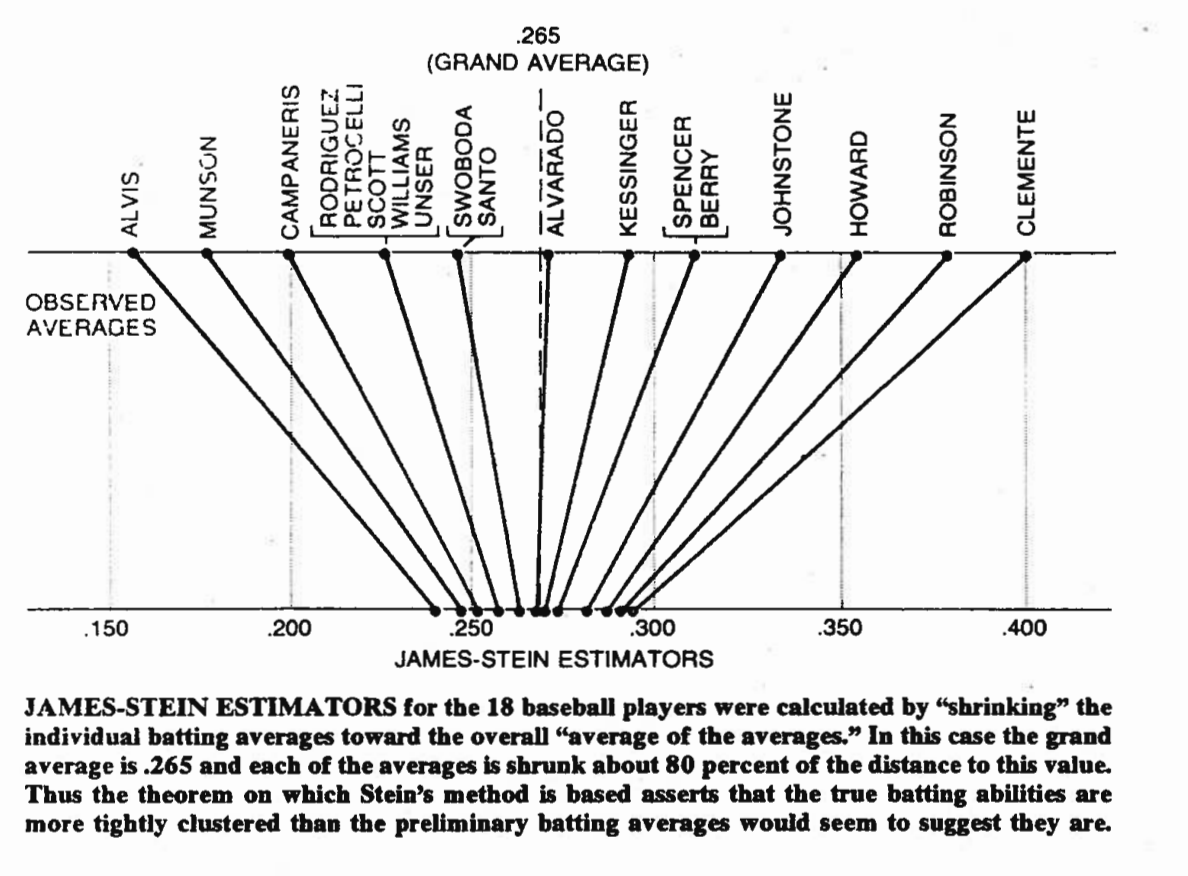
\includegraphics[scale=0.66]{week8_SteinsRegression}
    \end{center}

    Mathematically, note that since $Y_i \sim N(\theta_i, V)$ by assumption, it follows that
    \[
        Y_i = \theta_i + \sqrt{V}Z_i.
    \]
    It makes sense, then, that $\mathrm{Var} \left[Y_i \right] > \mathrm{Var} \left[\theta_i \right]$. \\

    Finally, see the R Code for simulations to test a $k=3$ case based on the Wordle example in previous problems. The code uses $\mu = 3.5$ and $V=1$, along with various values of $\theta_1$, $\theta_2$, and $\theta_3$. \\

    \item \textbf{Use data from the 2004 WNBA season to demonstrate the Stein estimate for $k = 13$.
    Let $y$ represent the average points scored for each team in their
    first $n = 5$ games, and $\theta$ represent the average for the remaining games in that season
    (a less noisy estimate of the underlying mean value). Imagine trying to predict the $\theta_i$'s based on the $Y_i$'s. 
    Estimate a common variance $V$ based on the team sample standard deviations and treat this as known for constructing the James-Stein estimates. Make a
    graph of $\theta$ vs $Y$, and draw in lines corresponding to using the $Y$ and $\hat{\theta}_i$'s. Add in the least squares line for fitting a straight line to estimate the $\theta_i$'s from the $Y_i$'s.
    Compare to the slope and intercept for the Stein estimate, along with the sums of squares about
    the $Y_i$'s, the $\hat{\theta}_i$'s, and about $\bar{Y}$.} \\

    See R Code. \\
    
    \item \textbf{Explain why shrinking the $Y_i$'s together seems like a sensible thing to do for the WNBA example, but may seem paradoxical in other situations. Use the Efron and Morris example of predicting batting averages, along with a proportion of foreign made cars. 
    Argue that using total squared error as a loss function means you are acting as if you have $k$
    related problems, and that this helps explain the apparent paradox.}\footnote{Details/wording taken from Phil's article on Stein's Paradox. Examples from Efron and Morris's Stein's Paradox article.} \\

    Efron and Morris often say the Stein estimate ``anticipates regression to the
    mean'' and improves the estimates by ``borrowing strength from the ensemble.''
    In the context of the baseball players, the ensemble (the collection of 18 players with 45 at-bats on a specific date
    in 1970) provides information about the distribution of batting averages in
    Major League Baseball that year. If we observed only one player's average, it
    would be equally likely to be an overestimate or an under-estimate of the
    player's true probability of getting a hit. But in the context of other similar players, we might reasonably judge a particular batting average is more likely to be
    an over-estimate or under-estimate. For example, Clemente's .400 was the largest of a sample of 18 batting averages.
    Without any outside knowledge that .400 is an unusually high average for a
    professional player, one could still judge that this was likely to be an over-estimate
    of Clemente's true probability. A classical confidence interval for Clemente's
    mean would be symmetric about .400,allowing for the possibility that he had
    a true probability larger than .400 and was in a batting slump for those first
    45 at-bats. The Stein estimate predicts Clemente to bat closer to the overall
    average $y =.265$, but still to be above average. Similarly, the Stein estimate predicts Max Alvis' final average to be higher
    than .156, but still below average. \\

    Similarly, shrinking the $Y_i$'s together in the WNBA example is essentially the idea of ``regressing to the mean''. \\

    What makes Stein's result more paradoxical is his general statement that,
when estimating a collection of $k$ (possibly unrelated) means using a set of independent sample averages, the averages
are inadmissible. That is, there is another estimate that does better (in terms of minimizing the sum of squares) for every possible set of means. The Stein estimate
was shown to be such an estimate. Efron and Morris illustrate the paradoxical nature of this fact by including a nineteenth average in their collection: the
percentage of a random sample of 45 foreign-made automobiles. Now, they
consider estimating the 18 player means and the overall percent of foreign-made
cars. Applying the Stein's estimate seems to imply that the percentage of foreign-made cars is influenced by the batting performances of Clemente and
the others. \\

\textit{But this is in fact not as paradoxical as one may think. With a simple regression model (to minimize the sum of squares),
the fitted value for the percent of foreign cars would be influenced by the batting
averages. The Stein estimate essentially attempts to fit this regression model
without having observed the responses, but assuming that they will be centered about the same mean as the predictors.}
\end{enumerate}
